

\chapter{Seven Segment Dsiplay}

\section{Introduction}

Seven segement display are one of the classical display units which are present in many electronics systems as shown in \autoref{fig:seven_seg:applications}.

\begin{figure}[h]
\centering
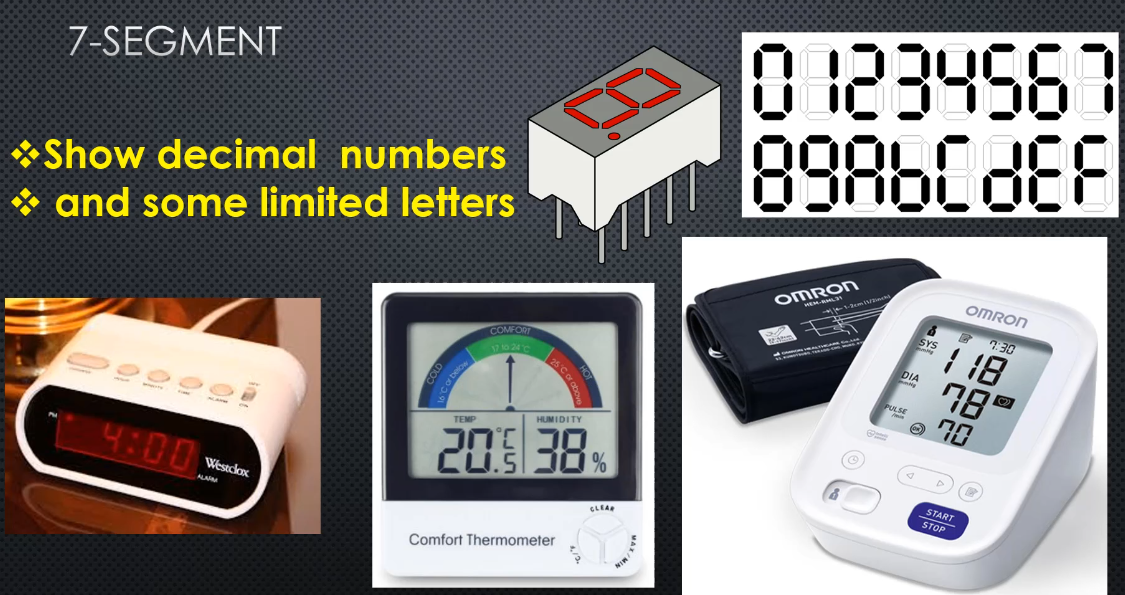
\includegraphics[scale=0.30,frame]{Figures/seven_seg/applications}
\caption{Seven segement presence in many electronic systems}
\label{fig:seven_seg:applications}
\end{figure}

In this chapter, we learn how to deal with these display using \verb|HLS|.\\

\newpage

\subsection{Driver}
\label{sub:Driver}

The driver for this type of display should contains 2 group of signals as shown in \autoref{fig:seven_seg:driver}:

\begin{itemize}

\item Data signal: control which number to be displayed

\item Control signal: select the target, that is which sgement we want to use.

\end{itemize}

\begin{figure}[h]
\centering
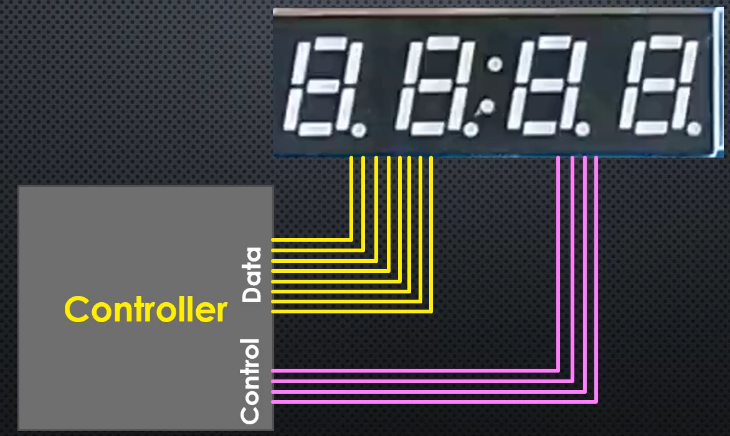
\includegraphics[scale=0.35,frame]{Figures/seven_seg/driver}
\caption{Signals for 7 segment}
\label{fig:seven_seg:driver}
\end{figure}


\underline{Notes regarding 7 Segement:}

\begin{itemize}

\item Multiple 7 segment share the same data signals and use them in a multiplex fashion managed by control signals.

\item The 7 segment uses a sequential circuit part, but in this chapter we focus on the combinational part, and explain some simple circuit and examples

\end{itemize}

\todo{7 Segment Notes:} \uti{7 Segment Notes:}

\begin{itemize}

\item \textit{To see what it does mean about the $\mathrm{1}^\mathrm{st}$ point above about sharing the same data signals} 

\item \textit{To be seen this later once I start reviewing the logic desing course and make the recap}

\end{itemize}

\newpage
\section{7 Segement Structure}
\label{sec:7seg_structure}

Now to dive into more technical details for 7 segment.\\

7 segment consist of 8 LED: 7 LED from A $\rightarrow$ G to display a digit, and 1 LED to display the digit point denoted as DP.

\begin{figure}[h]
\centering
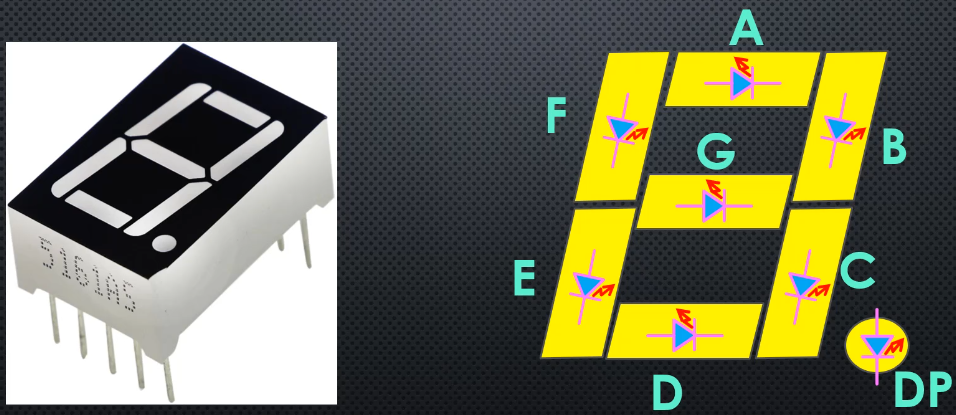
\includegraphics[scale=0.35,frame]{Figures/seven_seg/7seg_led}
\caption{7 segment LED structure}
\label{fig:seven_seg:7seg_led}
\end{figure}

7 segment has 2 types of connections: common anode and common cathode. In these configurations, multiple LED are connected together to a single point.


\begin{figure}[h]
\centering
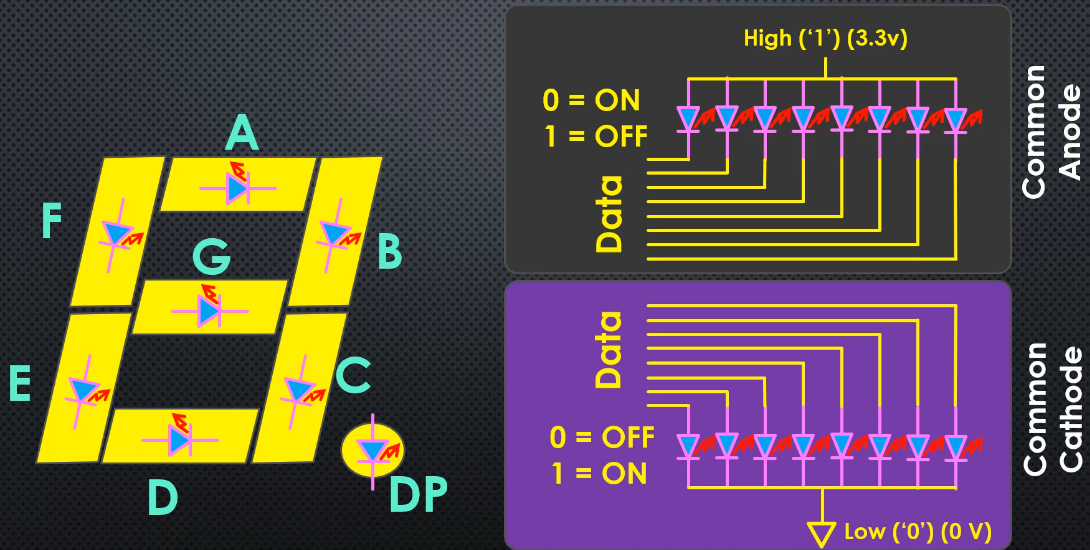
\includegraphics[scale=0.35,frame]{Figures/seven_seg/7seg_conf}
\caption{7 segment LED configuration: common anode and common cathode}
\label{fig:seven_seg:7seg_conf}
\end{figure}

\begin{itemize}

\item Common anode is where the $+$ side of the LED are connected to high voltage. In this configuration, a logic value of 0 turns the LED ON.

\item Common cathode is where the $-$ side are connected to low voltage. Therefore, a logic value of 1 turns a segment ON.

\end{itemize}


\newpage
\todo{Common Anode and cathode, insert in an appendix} \uti{Common Anode and cathode, insert in an appendix:}

\begin{itemize}

\item \textit{To make a review later about the circuit concept, like :}

	\begin{itemize}
	\item \textit{Common anode, cathode}
	
	\item \textit{Current flow,$\cdots$}
	\end{itemize}

\item \textit{To insert all these concepts in an appendix later}

\end{itemize}

To control a 7 segment regardless of the code which drives the 7 segment, a switch is used to turn ON or OFF the 7 segment. An example is shown in \autoref{fig:seven_seg:7seg_switch}.

\begin{figure}[h]
\centering
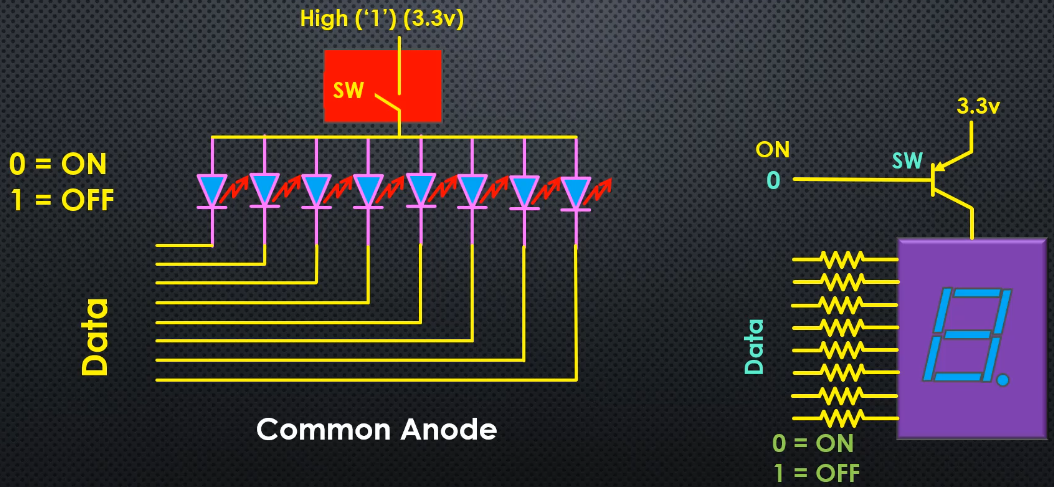
\includegraphics[scale=0.35,frame]{Figures/seven_seg/7seg_switch}
\caption{Switch control for a 7 segment using common anode configuration}
\label{fig:seven_seg:7seg_switch}
\end{figure}

\begin{itemize}

\item To turn ON the 7 segment, the switch should be driven by the logic value zero and

\item Proper data should be applied to the cathode

\end{itemize}

\newpage
\subsection{Quiz}

\underline{Quiz:} Find the logic values in the control and data signals to show the number 4 on this common anode 7 segment of \autoref{fig:seven_seg:quiz_7seg}.

\begin{figure}[h]
\centering
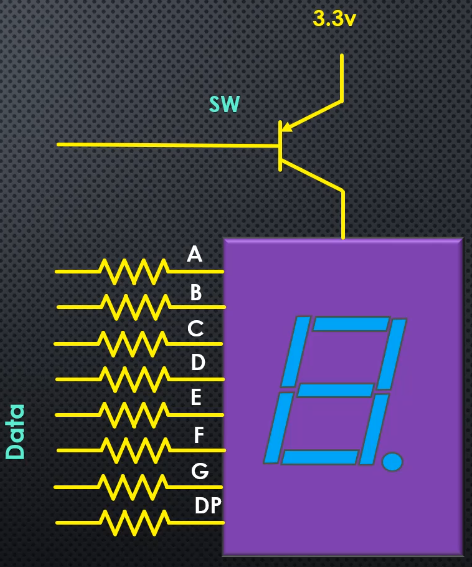
\includegraphics[scale=0.37,frame]{Figures/seven_seg/quiz_7seg}
\caption{Quiz 7 Segment}
\label{fig:seven_seg:quiz_7seg}
\end{figure}

\underline{Solution:}

\begin{itemize}

\item To turn on the 7-segment, the control signal connected to the PNP transistor switch should be 0.

\item To show the number 4, the data signal should turn on the LEDs on the four segments $B$, $C$, $F$ and $G$. So, as the 7-segment configuration is common anode the data is $0b10011001$

\end{itemize}

\begin{figure}[h]
\centering
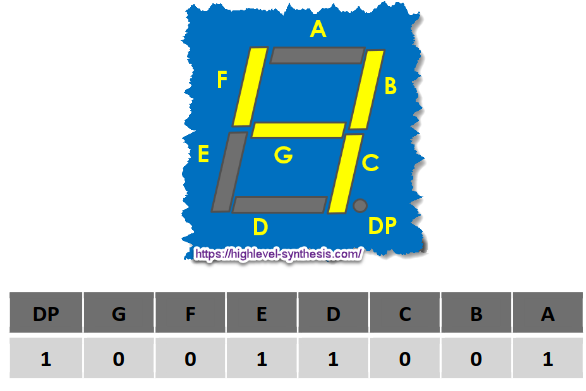
\includegraphics[scale=0.37,frame]{Figures/seven_seg/quiz_7seg_sol}
\caption{Quiz 7 Segment Solution}
\label{fig:seven_seg:quiz_7seg_sol}
\end{figure}

\newpage
\section{Digit Codes}
\label{sec:digit_codes}

\autoref{fig:seven_seg:anode_digit_codes} shows the different digit codes for common anaode configuration, where the control signal should be 0, and the data line also should be 0.

\begin{figure}[h]
\centering
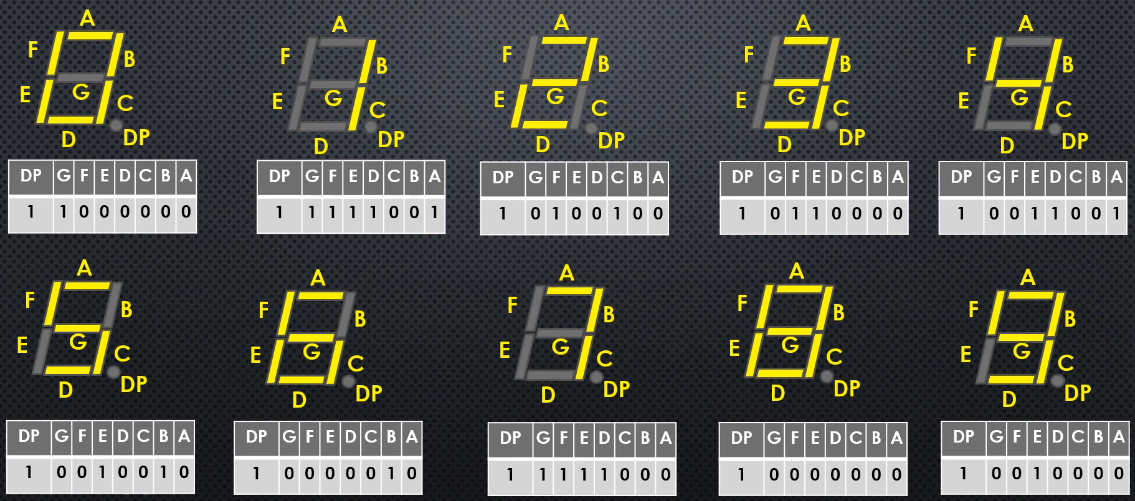
\includegraphics[scale=0.42,frame]{Figures/seven_seg/anode_digit_codes}
\caption{Digit codes for common anaode configuration}
\label{fig:seven_seg:anode_digit_codes}
\end{figure}

In a \verb|HLS| program, we can store these digit codes in an array and access them by their index as shown in \autoref{fig:seven_seg:codes_in_array}.


\begin{figure}[h]
\centering
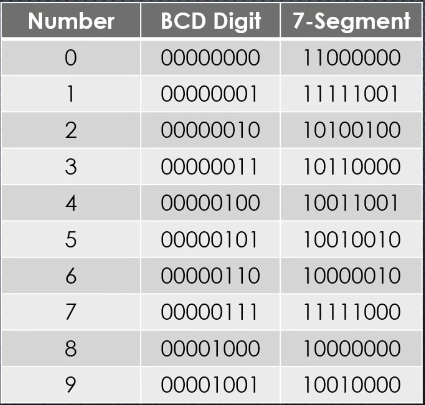
\includegraphics[scale=0.40,frame]{Figures/seven_seg/codes_in_array}
\caption{Digit codes stored in an array}
\label{fig:seven_seg:codes_in_array}
\end{figure}


\newpage
\section{7-Segment on Basys3}

After understanding general concepts of 7 segment circuit, we move to see the 7 segment on \verb|Basys3| board.\\


The \verb|Basys 3| board contains 4 segment display shown in \autoref{fig:seven_seg:basys3_7_seg}.

\begin{figure}[h]
\centering
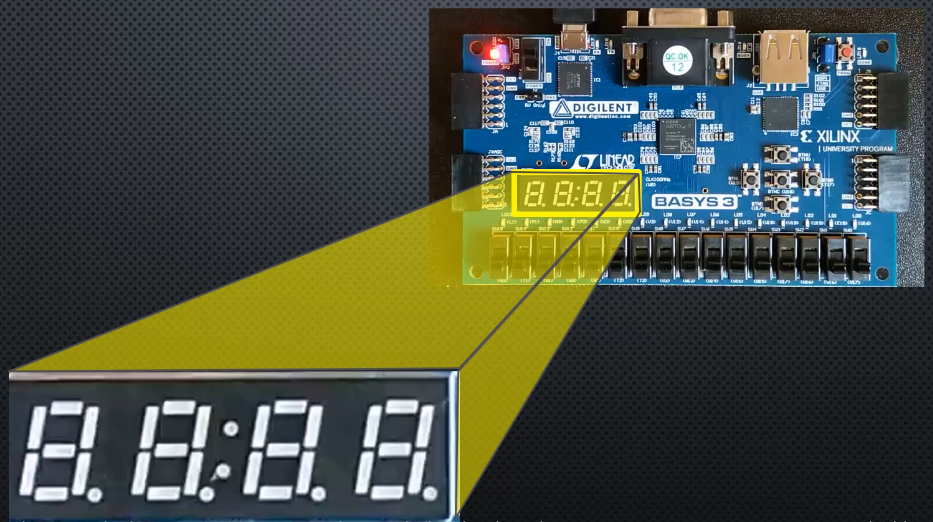
\includegraphics[scale=0.32,frame]{Figures/seven_seg/basys3_7_seg}
\caption{7 Segment on Basys 3}
\label{fig:seven_seg:basys3_7_seg}
\end{figure}

The pins configuration is shown in \autoref{fig:seven_seg:basys3_7seg_datasheet}.

\begin{figure}[h]
\centering
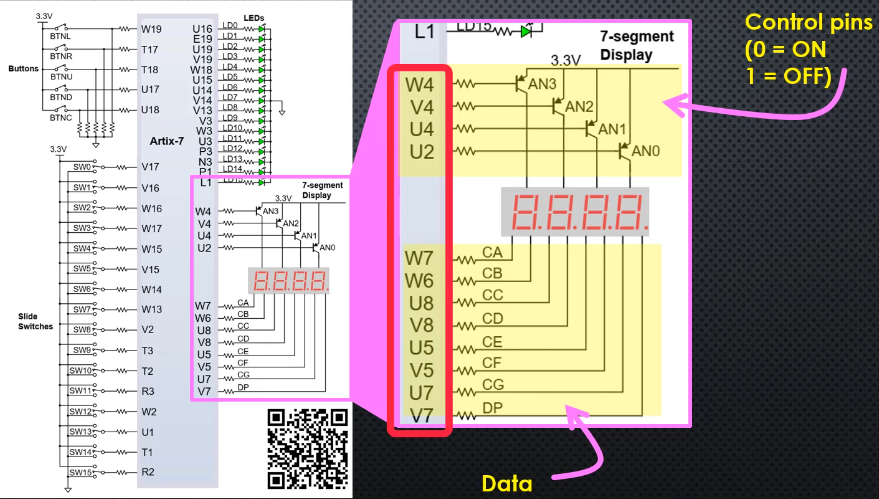
\includegraphics[scale=0.38,frame]{Figures/seven_seg/basys3_7seg_datasheet}
\caption{7 Segment pins configuration on Basys 3}
\label{fig:seven_seg:basys3_7seg_datasheet}
\end{figure}

\begin{itemize}

\item 12 pins are dedicated for the 4 7-seg:

	\begin{itemize}
	\item 4 pins for controls, where we have transistors acting a switch 
	
	\item 8 pins for data lines, shared among the 4 7-seg
	\end{itemize}

\item To display a digit using a 7-seg, and since the data lines are shared, \textit{time multiplexing} technique should be applied to the data signals

	\begin{itemize}
	\item Multiplexing requires a \textit{sequential desing}, which we will see in next chapters
	
	\item \todo{Multiplexing for 7 seg} \uti{Multiplexing for 7 seg:} \textit{To review this topic when started later in the sequential desing course}
	
	\item \textit{To cite the chapter later here}
	 
	\end{itemize}	   

\end{itemize}


\subsection{Quiz}

\underline{Quiz:} Find the control signal value and data code to write the number 5 on the left hand side 7 segment (according to \autoref{fig:seven_seg:basys3_7seg_datasheet}) and turn off the others.\\

\underline{Solution:}

\begin{itemize}

\item To enable the left-hand side display, we should apply 0 on W4 pin

\item To disable the others, V4, U4 and U2 should receive the logic value 1.

\item The code on the data pins is 0b10010010

\end{itemize}


\begin{figure}[h]
\centering
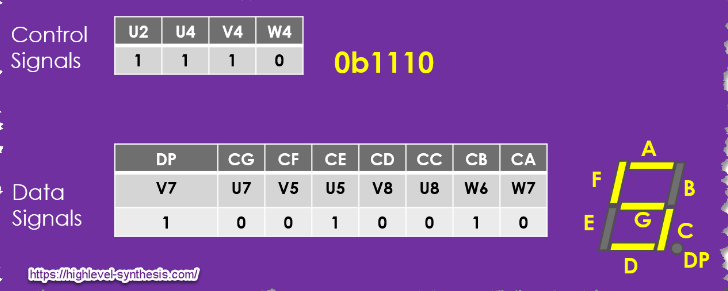
\includegraphics[scale=0.42,frame]{Figures/seven_seg/quiz_7seg_basys3_sol}
\caption{7 Segment quiz solution}
\label{fig:seven_seg:quiz_7seg_basys3_sol}
\end{figure}


\newpage
\section{1 Digit Example}

Now we take an example about 7 segment, and try implement it using \verb|HLS|. The given is shown in \autoref{fig:seven_seg:1digit_example}.

\begin{figure}[h]
\centering
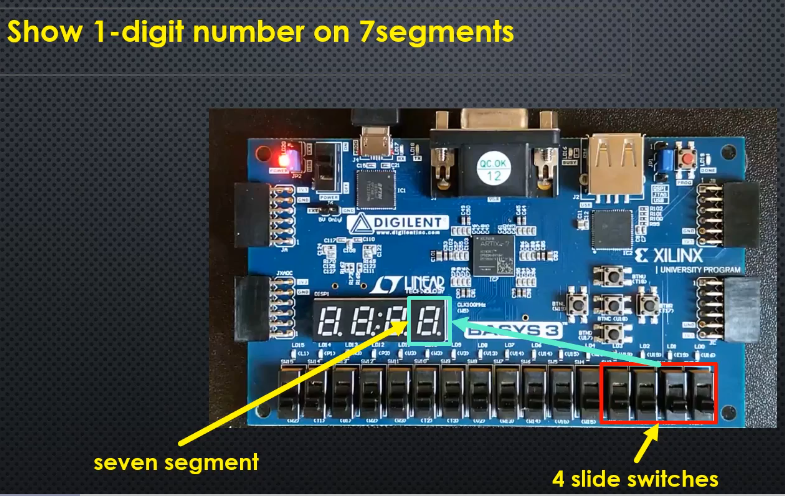
\includegraphics[scale=0.35,frame]{Figures/seven_seg/1digit_example}
\caption{Given of 1 digit example using 7 segment}
\label{fig:seven_seg:1digit_example}
\end{figure}

\subsection{Algorithm}

The algorithm that controls the 7 segment has 3 steps:

\begin{enumerate}

\item Get the digit binary code

\item Encoding the binary code into 7 segment code

\item Drive the target 7 segment display in the code

\end{enumerate}

These steps are illustrated in \autoref{fig:seven_seg:1digit_algo_step}.

\begin{figure}[h]
\centering
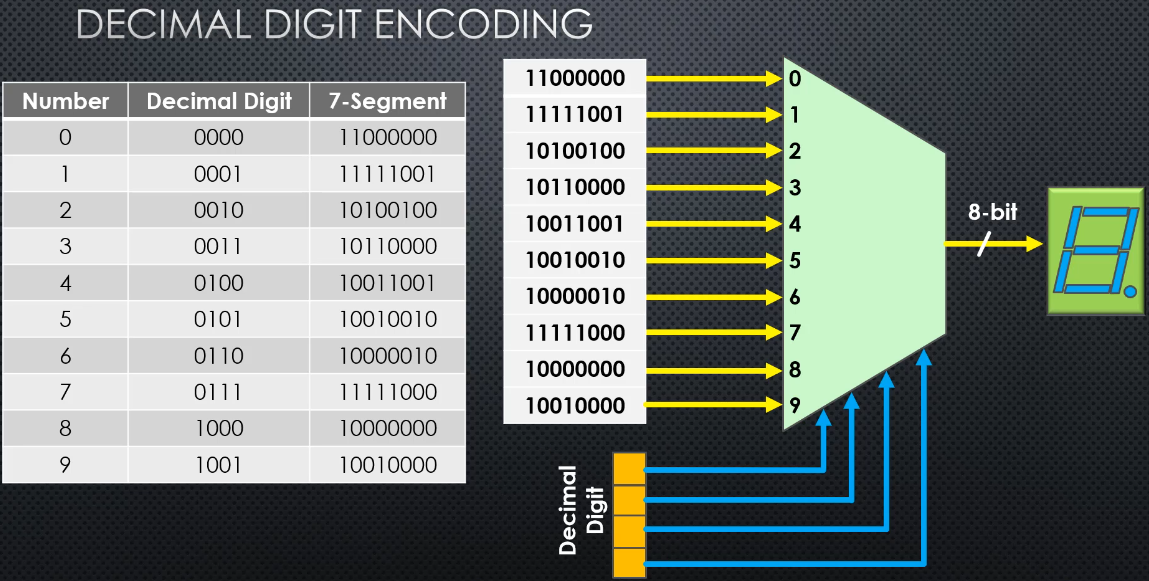
\includegraphics[scale=0.35,frame]{Figures/seven_seg/1digit_algo_step}
\caption{Steps of 1 digit algorithm display}
\label{fig:seven_seg:1digit_algo_step}
\end{figure}

\begin{itemize}

\item We have at the left side a table mapping the binary code of a digit to its corresponding 7 segment code

\item A MUX is used to encode binary representation of a digit into 7 segment code

	\begin{itemize}
	\item The binary code act as control signals for the MUX
	
	\item The 7 segment codes are input for the MUX
	\end{itemize}

\end{itemize}

\subsection{HLS Code}

The \verb|HLS| code is shown in \autoref{fig:seven_seg:1digit_hls}.

\begin{figure}[h]
\centering
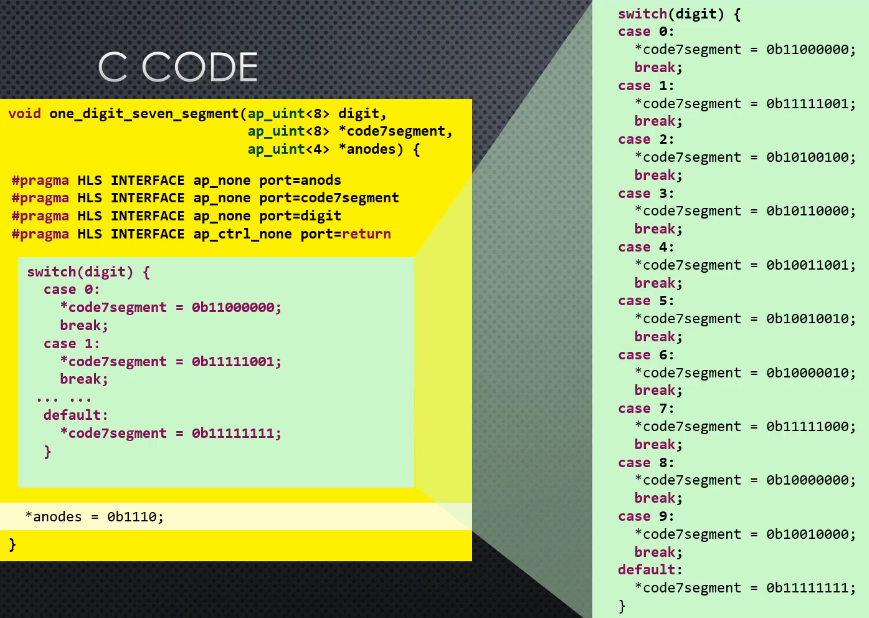
\includegraphics[scale=0.40,frame]{Figures/seven_seg/1digit_hls}
\caption{HLS code for 1 digit display}
\label{fig:seven_seg:1digit_hls}
\end{figure}

\newpage
\section{BCD Code}
\label{sec:BCD_code}

It is true that underlying computation in logic uses binary, but decimal number are more intuitive, this why BCD codes were invented, to make a transformation from binary to decimal, and display them in the 7 -seg.

The goal in this section is to see how to move from binary representation to BCD code, then display it on 7-seg.\\

Recall that a BCD for a number is \textit{the concatenation of its binary representation of its digit} . An example is shown in \autoref{fig:seven_seg:bcd_intro}, where we have the BCD of 24.

\begin{figure}[h]
\centering
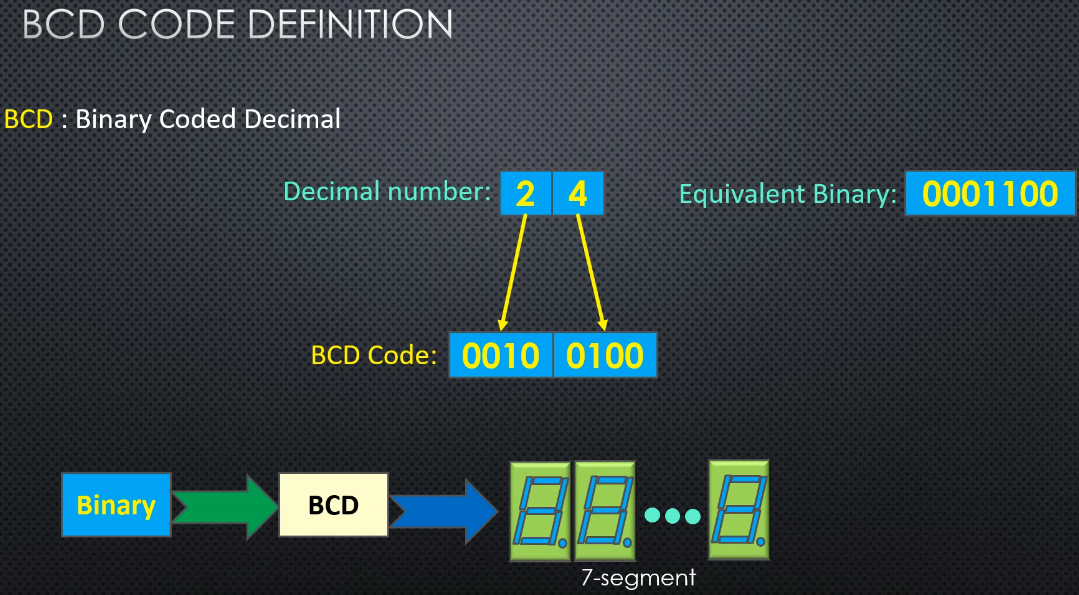
\includegraphics[scale=0.38,frame]{Figures/seven_seg/bcd_intro}
\caption{BCD definition}
\label{fig:seven_seg:bcd_intro}
\end{figure}

\newpage
\subsection{BCD Types and Memroy}

A 4 bit BCD can represent a decimal digit, but its saving in memory comes in different 2 different ways: packed and unpacaked. 

An example is shown in \autoref{fig:seven_seg:bcd_types}.

\begin{figure}[h]
\centering
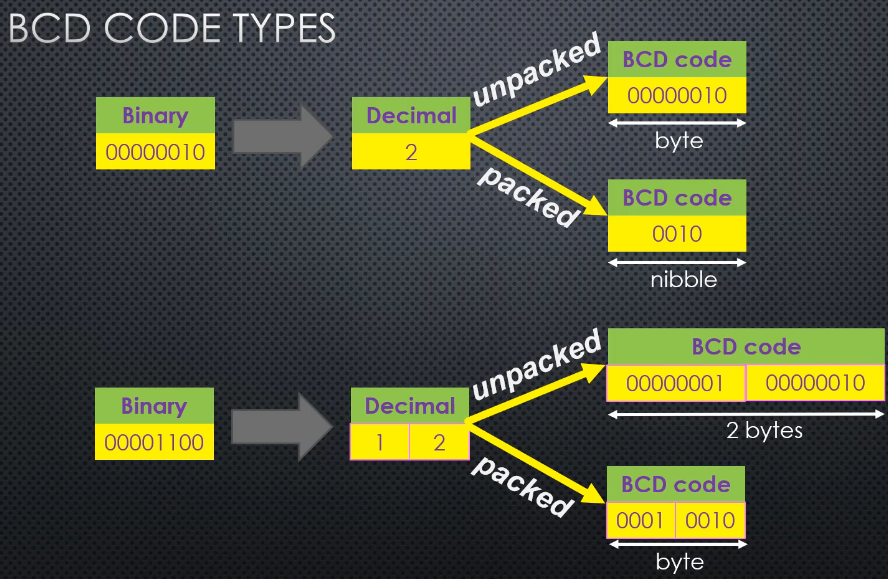
\includegraphics[scale=0.40,frame]{Figures/seven_seg/bcd_types}
\caption{BCD types}
\label{fig:seven_seg:bcd_types}
\end{figure}

\begin{itemize}

\item For the $\mathrm{1}^\mathrm{st}$ example, decimal 2:

	\begin{itemize}
	\item Unpacked version requires 8 bit, the upper 4 bit are all 0
		
	\item Packed version uses only 4 bit	
	\end{itemize}


\item For the $\mathrm{2}^\mathrm{nd}$ example, 12:

	\begin{itemize}
	\item Unpcaked requires 2 bytes of memory, since each digit require 8 bit (1 byte)
	\end{itemize}

\end{itemize}

\newpage
\subsection{Quiz}
\label{sub:binary_to_bcd}

\underline{Quiz:} Find the BCD code of the following binary number: 0b0001010001110100.\\


\underline{Solution:}\\

The decimal value of 0b0001010001110100 is 5 236. We take then the binary representation of each digit, and the BCD code will be the concatenation of each compact BCD digit as shown in \autoref{fig:seven_seg:qui_bcd_sol}.

\begin{figure}[h]
\centering
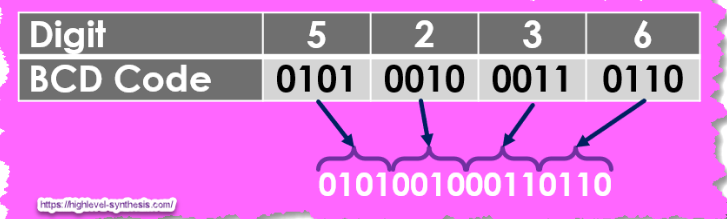
\includegraphics[scale=0.38,frame]{Figures/seven_seg/qui_bcd_sol}
\caption{BCD quiz solution}
\label{fig:seven_seg:qui_bcd_sol}
\end{figure}

\newpage
\section{HLS: Binary to BCD}
\label{sec:hls_binary_to_bcd}

Now our goal is to desing some combinational circuit using \verb|HLS| the convert some binary representation to BCD representation.\\

We study 3 methods to do such a conversion:

\begin{enumerate}

\item Modulo algorithm

\item A modified version of 1, withou a \verb|while| loop

\item The double dabble method, which uses shift operations and add 3

\end{enumerate}

\subsection{Modulo Method}

\autoref{fig:seven_seg:binary_to_bcd_hls} shows the algorithm along with some example in the right hand side

\begin{figure}[h]
\centering
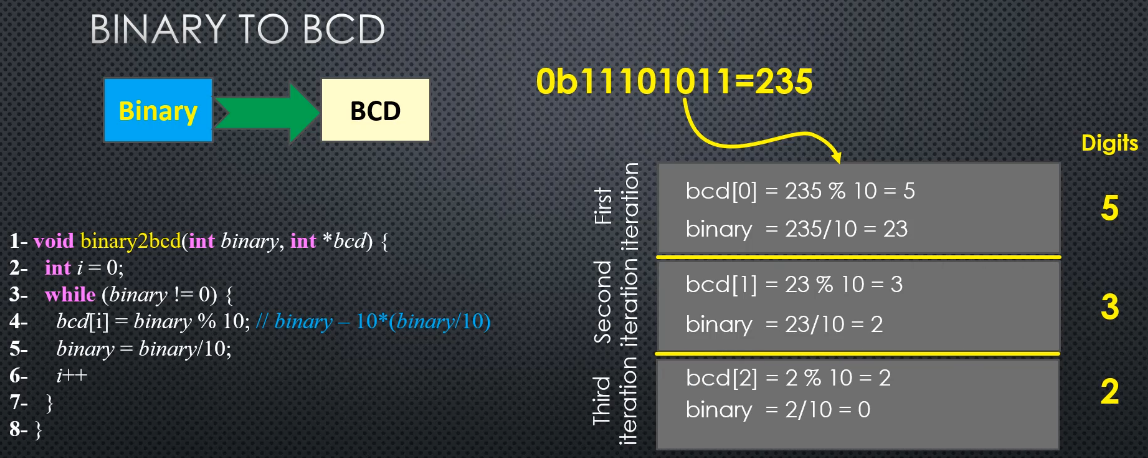
\includegraphics[scale=0.40,frame]{Figures/seven_seg/binary_to_bcd_hls}
\caption{Binary to BCD program}
\label{fig:seven_seg:binary_to_bcd_hls}
\end{figure}


\begin{itemize}

\item The input \verb|int binary| is 235

\item In the $\mathrm{1}^\mathrm{st}$ iteration, the algorithm extract the LSB digit from 235 using the \verb|%| operator

	\begin{itemize}
	\item Then it modifies the \verb|binary| by dividing by 10, so we can extract it the next digit in the next iteration
	\end{itemize}

\end{itemize}

The \verb|while| loop implies the usage of some sequential circuit, so we try to get rid of it (for now) and see how can we use some other approach.

\newpage
\subsection{Modified Algorithm}

Since we are working on \verb|Basys3| board which uses 4 7-segment, we assume that the number to be represented is in a range from $0 \, \rightarrow \, 9999$. \\

Also the \verb|while| loop of \autoref{fig:seven_seg:binary_to_bcd_hls} contains 2 arithmetic computation step, we will encapsulate these steps into some function and call this function 4 times (equal to 4 7-seg in \verb|Basys3|) board.

These modifications are shown in \autoref{fig:seven_seg:binary_to_bcd_modified}.

\begin{figure}[h]
\centering
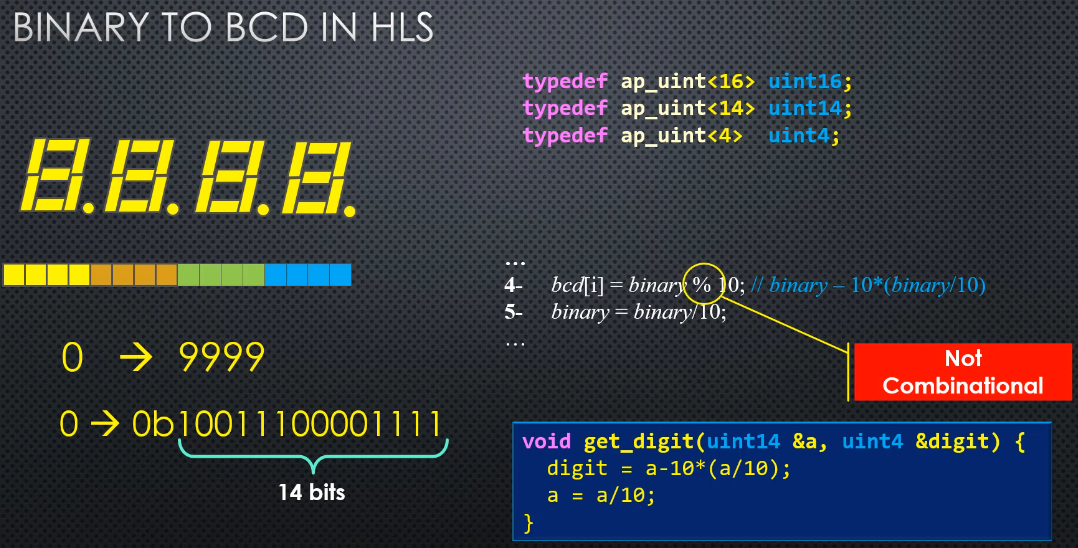
\includegraphics[scale=0.40,frame]{Figures/seven_seg/binary_to_bcd_modified}
\caption{Binary to BCD program modifications}
\label{fig:seven_seg:binary_to_bcd_modified}
\end{figure}

\begin{itemize}

\item For the data type

	\begin{itemize}
	\item for the input binary we need 14 bit number

	\item 4 bits to represent BCD code for a single digit			
 
	\item 16 bits to send out the BCD code to the 4 7-seg
	
	\end{itemize}

\item The \verb|%| operator is not in general a combinational circuit, so we use the equivalent statment \verb|a-10*(a/10)|

\end{itemize}

\newpage
The final code in \verb|HLS| using the modifications discusses above is shown in \autoref{fig:seven_seg:binary_to_bcd_modified_hls}.

\begin{figure}[h]
\centering
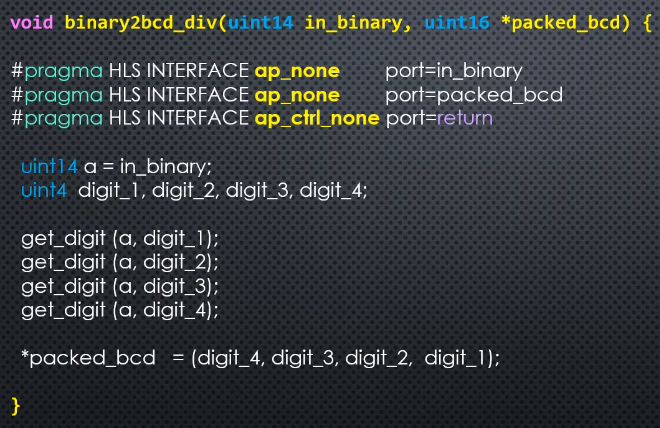
\includegraphics[scale=0.40,frame]{Figures/seven_seg/binary_to_bcd_modified_hls}
\caption{Binary to BCD program HLS code with modifications}
\label{fig:seven_seg:binary_to_bcd_modified_hls}
\end{figure}

\subsection{Double Dabble Algorithm}
\label{sub:double_dabble}

Now we explain a more efficient algorithm named \textit{double dabble}. This algorithm uses 2 operators: shift left and add 3.\\

\underline{Points of the algorithm:}

\begin{itemize}

\item We need a variable to store both binary and BCD numbers

	\begin{itemize}
	\item The variable should have enough space for both numbers
	\end{itemize}

\item 	The binary number is saved on the righ hand side of the variable, and BCD number (packed version) is hosted on the left side, and initialized to 0

	\begin{itemize}
	\item Recall for BCD number, we use 4 bits for each digit in packed version
	\end{itemize}

\item  For an $n$ bit binary number, the double dabble algorithm is perfomed $\left(\, n \, - \, 1 \, \right)$

\end{itemize}

\newpage
The steps of the algorithm in addition to a runnning example is shown in \autoref{fig:seven_seg:double_dabble_algo}.

\begin{figure}[h]
\centering
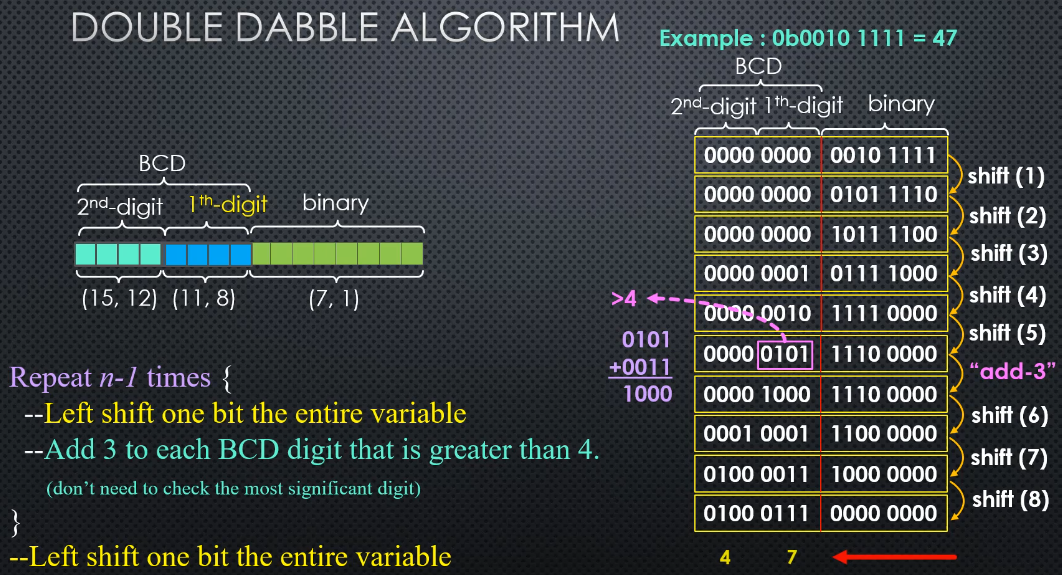
\includegraphics[scale=0.40,frame]{Figures/seven_seg/double_dabble_algo}
\caption{Binary to BCD using double dablle algorithm}
\label{fig:seven_seg:double_dabble_algo}
\end{figure}

\begin{itemize}

\item The input of the algorithm is 8 bit binary number, and 8 bit for the BCD code for 2 digit (4 bit for each digit)

\item After the $\mathrm{5}^\mathrm{th}$ shift, the $\mathrm{1}^\mathrm{st}$ BCD digit has a value of 5 ($> 4$). So we add 3 to it

\item Then we continue shifting to the left the rest of the binary variable

\end{itemize}

The \verb|HLS| code is shown in \autoref{fig:seven_seg:double_dabble_hls}.

\begin{figure}[h]
\centering
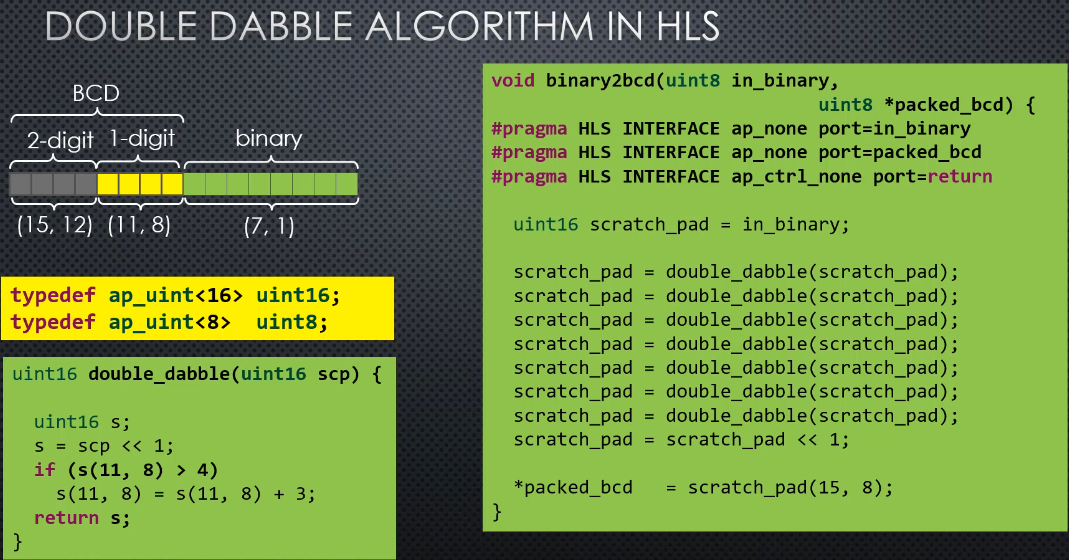
\includegraphics[scale=0.40,frame]{Figures/seven_seg/double_dabble_hls}
\caption{Double dablle algorithm in HLS}
\label{fig:seven_seg:double_dabble_hls}
\end{figure}


\newpage
\section{2 Digit Code}

Afer seeing the algorithm that turns a binary number to a BCD code, we move to the implementation on \verb|Basys3| board, and try to display 2 digit code.\\

Tha approach is shown in \autoref{fig:seven_seg:bcd_2_digit}.

\begin{figure}[h]
\centering
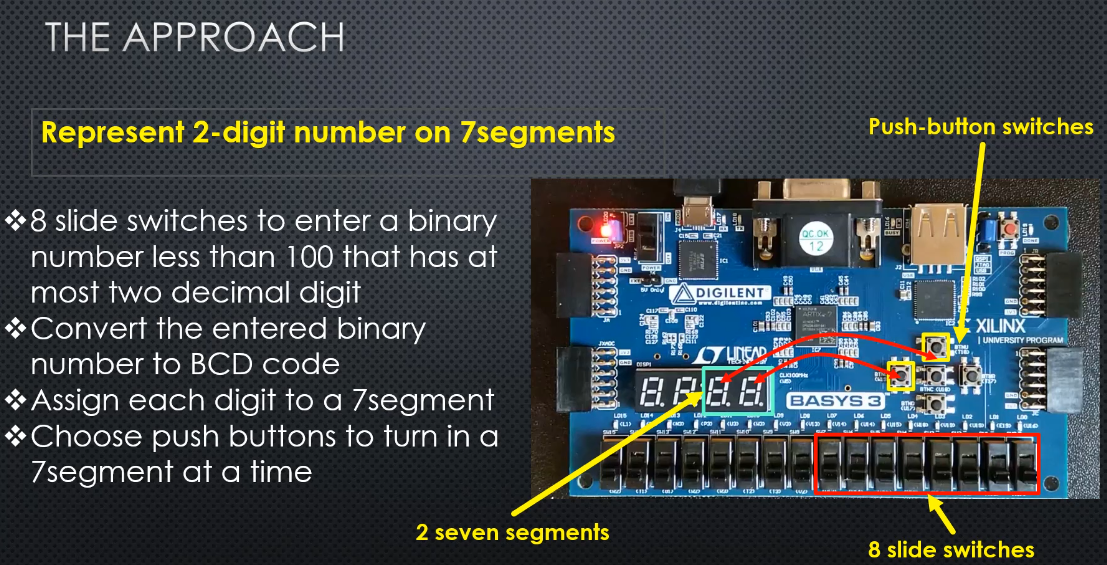
\includegraphics[scale=0.40,frame]{Figures/seven_seg/bcd_2_digit}
\caption{BCD for 2 digit on Basys3 FPGA}
\label{fig:seven_seg:bcd_2_digit}
\end{figure}

The steps and the \verb|HLS| code is shown in \autoref{fig:seven_seg:bcd_2_digit_steps_hls}.

\begin{figure}[h]
\centering
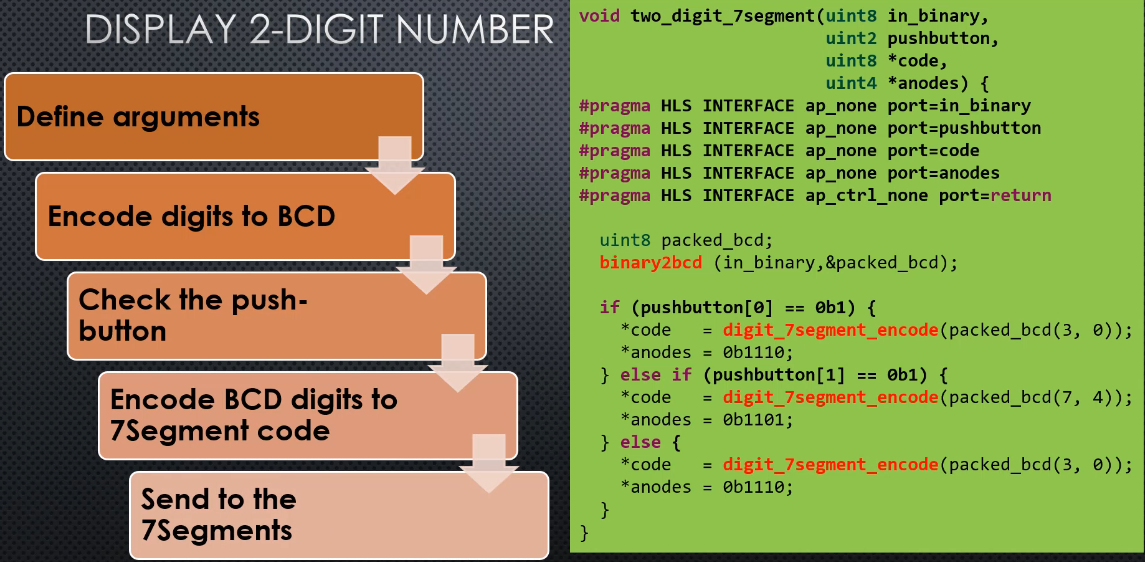
\includegraphics[scale=0.40,frame]{Figures/seven_seg/bcd_2_digit_steps_hls}
\caption{BCD for 2 digit steps and HLS code}
\label{fig:seven_seg:bcd_2_digit_steps_hls}
\end{figure}

\newpage
\subsection{Quiz}

\underline{Quiz:} Write an \verb|HLS| code to show a 4 digit number on 7-segments. Use push button as shown in \autoref{fig:seven_seg:quiz_4_digit} to activate each 7 segment.

\begin{figure}[h]
\centering
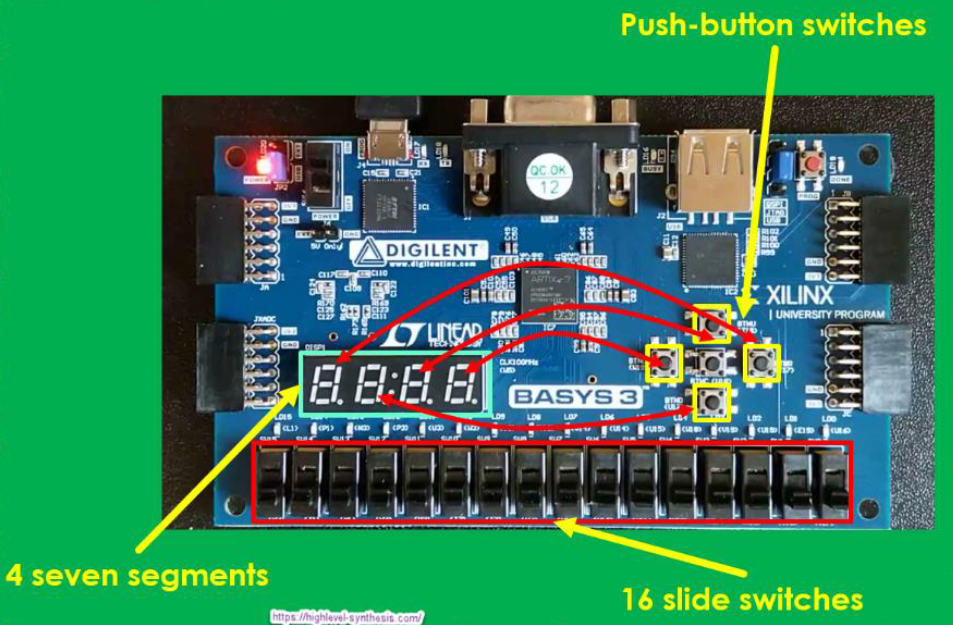
\includegraphics[scale=0.33,frame]{Figures/seven_seg/quiz_4_digit}
\caption{Push buttons mapping to active 7 segment}
\label{fig:seven_seg:quiz_4_digit}
\end{figure}

\underline{Solution:} The \verb|HLS| code is shown in \autoref{fig:seven_seg:quiz_4_digit_sol}.

\begin{figure}[h]
\centering
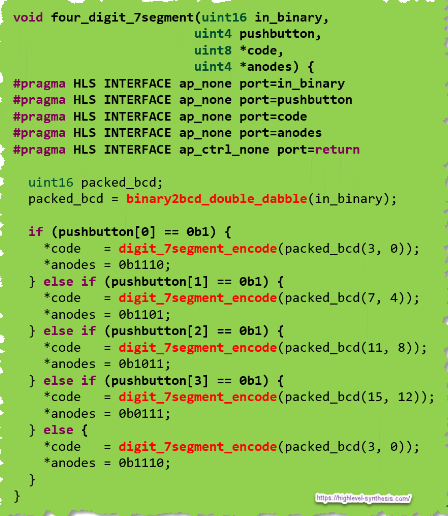
\includegraphics[scale=0.48,frame]{Figures/seven_seg/quiz_4_digit_sol}
\caption{Push buttons mapping to active 7 segment}
\label{fig:seven_seg:quiz_4_digit_sol}
\end{figure}


\newpage
\section{Exercices}

\todo{7Seg Ex} \uti{7Seg Ex:}

\begin{itemize}

\item \textit{To do these exercices later}

\item \textit{Insert comment and solution in readme file or the report}

\end{itemize}

\begin{enumerate}

\item Design a logic circuit that receives a four-digit compact BCD code and returns its equivalent binary value.

\item Show a four-digit hex number on the 7-segments available on the Basys3 board. Use the slide switches to enter the number. In addition, use the pushbuttons as shown in \autoref{fig:seven_seg:ex_2_7seg} to activate a 7-segment at a time.

\begin{figure}[h]
\centering
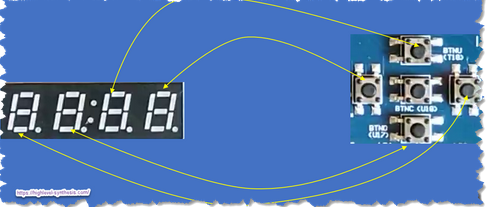
\includegraphics[scale=0.48,frame]{Figures/seven_seg/ex_2_7seg}
\caption{Exercie 2 given}
\label{fig:seven_seg:ex_2_7seg}
\end{figure}

\item Design a logic circuit that gets the ASCII codes corresponding to the lower-case letters a, b, c, d, e, f, g, h, l and show them on a right-hand side 7-segment. Use the slide switches to enter an ASCII code. \autoref{fig:seven_seg:ex_3_table} shows the ASCII codes for these letters.

\begin{figure}[h]
\centering
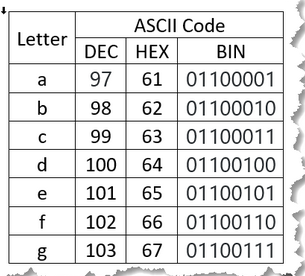
\includegraphics[scale=0.48,frame]{Figures/seven_seg/ex_3_table}
\caption{Exercie 3 ASCII table}
\label{fig:seven_seg:ex_3_table}
\end{figure}


\end{enumerate}



\newpage
\section{Summary}

\begin{itemize}

\item Signals for 7-Seg (\ref{sub:Driver})

	\begin{enumerate}
	\item Control signal $\leftrightarrow$ segment selection 
	
	\item Data signal $\leftrightarrow$ digit value
	\end{enumerate}

\item Configuration (\ref{sec:7seg_structure}):

	\begin{itemize}
	\item Common anode: $+$ side of LED to high voltage, and logic 0 turn LED ON
	
	\item Common cathode: $-$ side of LED to ground, and logic 1 to turn LED ON
	
	\item \autoref{tab:7seg_conf} group these configuration
	
	\begin{table}[h!]
\centering

\begin{tabular}{|c|c|c|}
\hline
Configuration & Common Anode & Common Cathode \\
\hline
Shared terminal & All anodes to Vcc & All cathodes tied to GND \\ \hline
\multirow{2}{*}{Segment control} & Each segment has its own cathode  & Each segment has its own anode  \\ \cline{2-3}
& separate cathode & separate anode \\ \hline
Turn ON segment (LED) & Logic 0 & Logic 1  \\ \hline
FPGA boards & Basys3 & \\ \hline
\end{tabular}
\caption{Comparison of Common Anode vs Common Cathode LED configurations}
\label{tab:7seg_conf}
\end{table}
	
	 
	\end{itemize}

\item BCD codes (\ref{sec:BCD_code})

	\begin{itemize}
	\item Single digit (as in 4): same as binary representation 
	
	\item multiple digit (as 47): concatenation of binary code for each digit
	
	\item From binary to BCD (\ref{sub:binary_to_bcd}):
	
		\begin{enumerate}
		\item get back to decimal
		
		\item Take each digit in binary representation form
		
		\item Concatenate the result
		\end{enumerate}
	
	
	\end{itemize}

\item Binary to BCD (\ref{sec:hls_binary_to_bcd}): 

This section contains method to transform a binary number into its BCD code. 


\item  We recap the double dabble algorithm (\ref{sub:double_dabble}):

Take as example an $n \, = \, 8 $ bit binary \verb|0b0010 1111| ($= 47$).

For $ n -1$ times (that is 7 in our case): 

\begin{itemize}

\item we shift by 1 the binary number

\item We check if the BCD part if greater than 4, we add 3

\end{itemize}

After finishing the $n \, - \, 1$ iterations, we shift by 1 one last time for the MSB part.

\end{itemize}

\newpage
A summary about the steps learned in 7-seg is shown in \autoref{fig:seven_seg:summary_7seg}.

\begin{figure}[h]
\centering
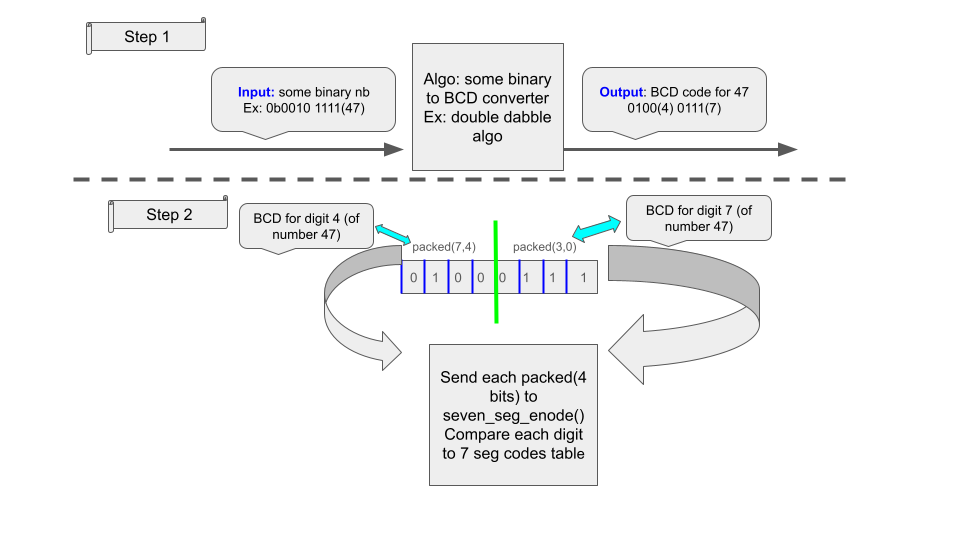
\includegraphics[scale=0.52,frame]{Figures/seven_seg/summary_7seg}
\caption{Summary for 7 Seg}
\label{fig:seven_seg:summary_7seg}
\end{figure}